\section{Structured Prediction}
% don't need very details of the algorithm
% need problem definition
% copied from nips paper
Travel route recommendation problems involve a set of POIs in a city. 
Given a trajectory query $\mathbf{x} = (s, l)$, comprising a start POI $s$ and trip length $l$, the goal is to suggest one or more sequences of POIs that maximise some notion of utility.

We first cast travel recommendation as a structured prediction problem, which allows us to leverage the well-studied literature of structured SVMs (SSVM)~\cite{tsochantaridis2005large,joachims2009predicting}. 
There are two obstacles that prevent us from applying SSVM directly to the sequence recommendation problem; first, there would be multiple ground-truth routes among a set of POIs, second, a naive application of SSVM would generate a loop during prediction time. 
To incorporate multiple ground-truth routes in the learning phase, we take an idea from the ranking objective which prevents the ground-truth routes from competing with each others~\cite{rendle2009bpr}. 
To eliminate possible loops in prediction, we adopt the serial list Viterbi algorithm~\cite{seshadri1994list,nill1995list,nilsson2001sequentially}.
We finally trained our model on trajectory data extracted from Flickr photos taken in Melbourne~\cite{chen2016learning}.

From a visualisation perspective, an important advantage of the SSVM is the explicit representation of feature scores in its final decision process. Especially, in our case, we can disassemble the final score of a route into feature scores of each POI and each transition between two adjacency POIs. 
We use hand-crafted POI features such as the category, popularity, and average visit duration of previous tourists and also crafted transition features such as the distance and neighbourhood of two POIs to maximise the interpretability of the outcome.

\begin{figure}[t!]
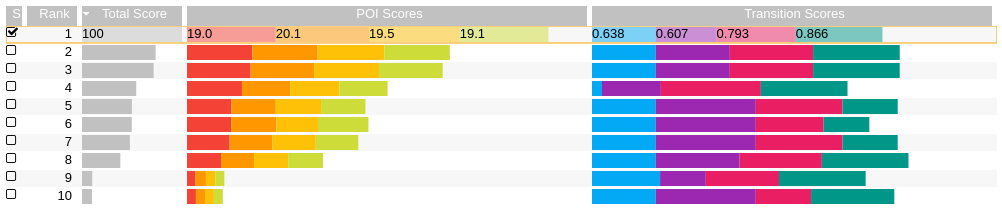
\includegraphics[width=0.8\linewidth]{figure/sample_stack.png}
\caption{Visualisation of POI scores for top ten recommended routes. Each bar from left to right represent a relative score of each POI along the route, and the total length of stacked bars represents the total score of the suggested route.}
\label{fig:stack}
\end{figure}